\documentclass[conference]{IEEEtran}
\IEEEoverridecommandlockouts
% The preceding line is only needed to identify funding in the first footnote. If that is unneeded, please comment it out.
\usepackage{cite}
\usepackage{amsmath,amssymb,amsfonts}
\usepackage{algorithmic}
\usepackage{graphicx}
\usepackage{textcomp}
\usepackage{xcolor}
\usepackage{algorithm} 
\usepackage{algorithmic}
\usepackage{graphicx}
\usepackage{subcaption}
\usepackage{textcomp}
\usepackage{url}
\usepackage[utf8]{inputenc}
\usepackage{lipsum} % Required to insert dummy text
\usepackage[version=4]{mhchem}
\usepackage{siunitx}
\usepackage{tikz}

\def\BibTeX{{\rm B\kern-.05em{\sc i\kern-.025em b}\kern-.08em
		T\kern-.1667em\lower.7ex\hbox{E}\kern-.125emX}}
\begin{document}
	
	\title{A Comparison of Stochastic Gradient MCMC using Multi-Core and GPU Architectures}
	
	\author{
	\IEEEauthorblockN{Sergio Hern\'andez}
	\IEEEauthorblockA{Laboratorio de Procesamiento de Informaci\'on Geoespacial.\\ Universidad Cat\'olica del Maule. Chile. shernandez@ucm.cl}
	\and
	\IEEEauthorblockN{Jos\'e Vald\'es}
	\IEEEauthorblockA{ Centro de Innovaci\'on en Ingenier\'ia Aplicada.\\  Universidad Cat\'olica del Maule. Chile.}
	\and
	\IEEEauthorblockN{Matias Valdenegro}
	\IEEEauthorblockA{ German Research Center for Artificial Intelligence.\\ Robotics Innovation Center. Germany.}
	}
	
	\IEEEoverridecommandlockouts
	\IEEEpubid{\makebox[\columnwidth]{978-1-7281-9716-6/20/\$31.00~\copyright2020 IEEE \hfill} \hspace{\columnsep}\makebox[\columnwidth]{ }}
	\maketitle
	\IEEEpubidadjcol
	\begin{abstract}
		Deep learning models are traditionally used in big data scenarios. When there is not enough training data to fit a large model, transfer learning re-purpose the learned features from an existing model and re-train the lower layers for the new task. Bayesian inference techniques can be used to capture the uncertainty of the new model but it comes with a high computational cost. In this paper, the run time performance of an Stochastic Gradient Markov Chain Monte Carlo method using two different architectures is compared, namely GPU and multi-core CPU. As opposed to the widely usage of GPUs for deep learning, significant advantages from using modern CPU architectures.
	\end{abstract}
	
	\begin{IEEEkeywords}
		Bayes methods, Monte Carlo methods, Stochastic Gradient MCMC
	\end{IEEEkeywords}

\section{Introduction}
As the amount of stored data is increased. analytical techniques for processing large-scale datasets are also required. In the other hand, big datasets are not only described by the number of observations but also through its dimensionality (number of features). Therefore. modern scalable Bayesian inference techniques must be able to improve performance on a single machine (scale up) as well as distributing performance across several machines or CPU cores (scale out) \cite{angelino2016patterns}.

In particular. Bayesian inference is used for computing posterior distributions of the model parameters. In order to obtain such posterior estimates. Markov Chain Monte Carlo (MCMC) methods approximate intractable integrals as an expectation using a finite number of samples. However, this expectation requires the full dataset in order to guarantee convergence.  Splitting a big dataset into smaller batches and running parallel chains is a simple alternative for scaling out Bayesian inference. Nevertheless, each chain will have its own posterior approximation and there is no standard method for recombining the results into a single posterior distribution. 

The Stochastic Gradient Langevin Monte Carlo (SGLD) algorithm is an approximation technique that fully exploits data subsets \cite{welling2011bayesian}. The method replaces gradients and likelihood evaluations required by standard MCMC by stochastic gradients based on data subsets (mini-batches). Some implementations can be found in software libraries such as Edward \cite{Tran2018}, ZhuSuan \cite{zhusuan2017} and the SGMCMC package \cite{baker2017sgmcmc}. All of these implementations are based on TensorFlow\footnote{\url{https://www.tensorflow.org/}} as a backend and therefore inherit the scalability of GPU computation. However, there is little research done on the scalability of SGLD using modern CPU architectures. Therefore, this paper presents a novel comparison of SGLD implementations on GPUs and CPUs. 
% 
\subsection{Related work}
Deep learning research has attracted a lot of attention from practitioners and industry. Therefore, most modern models require specific hardware accelerators such as GPUs and multi-core CPUs. Benchmark suites such as BenchIP \cite{Tao2018} and BenchNN \cite{Chen2012} have been proposed for the task of hardware evaluation for neural networks. However, there is little research done on the scalability of SGLD using modern CPU architectures. 

\section{Stochastic Gradient MCMC}
Stochastic Gradient Descent (SGD) is an optimization technique traditionally used for out-of-core training deep learning models. Let $\mathbf{D}=\{\mathbf{d_1},\ldots,\mathbf{d_N}\}$ represent a typical dataset used for classification problems, as a set of tuples $\mathbf{d}=(\mathbf x,y)$ that contains features $\mathbf x \in \mathbb R^D$ and labels $y=\{1,\ldots,K\}$. Conversely, the stochastic optimization procedure iterates  over mini-batches of size $B \ll N$ and computes a point estimate $\theta^\ast = \operatorname{argmax} p(\mathbf{D} \vert \theta)$.

Deep learning models such as convolutional neural networks may exploit model parallelism for fully connected layers and data parallelism for convolutional layers. The former training technique applies parallelism across the model dimension (number of features) and the latter technique applies parallelism across the data dimension (number of examples). In a model parallel setting, different workers are trained on the same batch and they recombine results as soon as possible. In the other hand, in a data parallel setting, each worker is trained on different batches of data \cite{LI201695}. 

In the Bayesian framework, the unknown parameter $\theta$ is considered as a random variable. The Stochastic Gradient Langevin Monte Carlo (SGLD) algorithm uses an stochastic gradient approximation to generate samples from the posterior distribution $p(\theta \vert \mathbf{D})$. The SGLD algorithm generate proposals using:

\begin{align}
\theta_{t+1}=\theta_{t}+\frac{\epsilon_t}{2}\Big(\nabla\operatorname{log}p(\theta_{t})+\frac{N}{B} \sum_i^B \nabla \operatorname{log} p(\mathbf{d_i} \vert \theta_{t})\Big) + \eta_t
\label{eq:sgld}
\end{align}

where $\eta_t \sim \mathcal N(0,\epsilon_t)$ and $\epsilon_t \mapsto 0$ is a time-decaying step size.

It is important to notice that using SGLD on a fully connected layer requires dense matrix multiplications for computing the log-likelihood and the log-prior. 

\subsection{GPU SG-MCMC}
Graphic Processing Units (GPus) are many-core processors that offer massively parallel computation. GPUs are well suited for data parallel operations such as computing the gradient in convolutional neural networks and Monte Carlo methods \cite{lee2010utility}. In order to implement the SGLD algorithm, a Python library for GPU computation is used \footnote{\url{https://cupy.chainer.org/}}. The library includes optimized GPU array manipulation and linear algebra routines, which are compatible with other CPU array manipulation routines such as Numpy. 
 
 
\begin{figure}
	\centering
	\begin{subfigure}[b]{0.4\textwidth}
		
\includegraphics[width=\textwidth]{figures/cpu_architechture}
		\caption{CPU implementation.}
		\label{fig:cpuarchitechture}
	\end{subfigure}
	~ %add desired spacing between images, e. g. ~, \quad, \qquad, \hfill etc. 
	%(or a blank line to force the subfigure onto a new line)
	\begin{subfigure}[b]{0.4\textwidth}
		
\includegraphics[width=\textwidth]{figures/gpu_architechture}
		\caption{GPU implementation.}
		\label{fig:gpuarchitechture}
	\end{subfigure}
	\caption{SG-MCMC implementation on CPU and GPU. In CPU, a data queue feeds multiple Markov chains. In GPU, a single mini-batch is fed to a Markov chain that updates model parameters.}\label{fig:sgld_architechture}
\end{figure}
 
 
\subsection{CPU SG-MCMC}
Modern CPUs are equipped with multiple cores which are well suited to single instruction multiple data operations. The Python programming language is built around a Global Interpreter Lock, which prevents the execution of multiple threads at once.  Nevertheless, parallel Markov can be spawn using all available cores.  Moreover, data parallelism can be achieved by sharing a data queue that feeds each process with a different data mini-batch.  Figure \ref{fig:sgld_architechture} depicts the proposed GPU and CPU implementations of the SGLD algorithm. 


\section{Experimental results}
Serial versions of the SGD and SGLD algorithms are tested on CPU and compared with parallel
implementations on GPU. All experiments are run on a server with an Intel Xeon E5-2620 CPU
with 12 cores using a single fully connected softmax layer (which is widely used in transfer learning).
The server is also equipped with an NVIDIA TITAN X GPU and both implementations were developed
using Python 3.4.9.

\subsection{Synthetic data}
In this section, the goal is to demonstrate performance and scalability of the SGLD algorithm. The GPU and CPU implementations are tested using randomly generated multi-class classification problems. Different combinations on the number of features $D$ and number of instances $N$ were tested. The number of classes was set to $K=3$, the number of epochs was set to $E=2 \times 10^4$ and the size of the mini-batches was set to $B=50$ for all examples.

Firstly, a serial version  of the SGD algorithm is tested on the CPU and compared with a parallel implementation on the GPU. All experiments are run on a Server with an Intel Xeon E5-2620 CPU with 12 cores using a single fully connected softmax layer (which is widely used in transfer learning). Table \ref{tab:sgd} shows the run time for the different values of $D$ and $N$. According to \cite{LI201695}, convolutional layers contain $90\%$ of the computation and $5\%$ of the parameters, while fully connected layers contain $95\%$ of the parameters and $5\%-10\%$ of the computation. Consistently, since there is a fully connected layer operating on a small batch of data, there is no speedup and the GPU implementation is about $10$x slower than the CPU implementation.

\begin{table}[h]
	\centering
 \begin{tabular}{|c|c|c|c|c|c|c|}
 	\hline 
 	D & N & CPU Time [s] & GPU Time [s]  & Speed-Up\\ 
 	\hline 
 	10 &	1000&	11.98&	124.85& 10.42\\
 	10&	10000&	119.90&	1245.98& 10.39\\
 	10&	50000&	594.71&	6186.05& 10.40\\
 	10&	100000&	1195.62&	12261.716& 10.25\\
 	\hline
 	50&	1000&	13.67&	123.13& 9.00\\
 	50&	10000&	135.96&	1230.19& 9.04\\
 	50&	50000&	689.89&	6137.79& 8.89\\
 	50&	100000&	1487.26&	12240.06& 8.22\\
 	\hline
 	100&	1000&	15.71&	123.53& 7.86\\
 	100	&10000&	156.94&	1231.121& 7.84\\
 	100&	50000&	806.78&	6176.91& 7.65\\
 	100&	100000&	1770.83&	12394.13& 6.99\\
 	\hline 
 \end{tabular}
\caption{Run time comparison of CPU and GPU implementations of SGD for a softmax regression problem}
\label{tab:sgd} 
\end{table}
 
Secondly, the run time behavior of a multi-core CPU implementation of SGLD is shown in Table \ref{tab:sgld}. Similar to SGD, run time is scales with the number of data points $N$ and features $D$. This is not the case of the GPU implementation of SGD, where the number of features seems not to affect the run time due to the massive parallel processing capabilities of the GPU.

\begin{table}[h]
	\centering
	\begin{tabular}{|c|c|c|c|c|c|c|}
		\hline 
		D & N & CPU Time [s] & GPU Time [s]  & Speed-Up\\ 
		\hline 		
10	& 1000& 	24.75& 294.04  & 11.87\\
10	& 10000& 	245.22& 2946.67	& 12.01\\
10	& 50000& 	1186.81& 14518.66 & 12.23\\
10	& 100000	& 2380.18& 29010.43& 12.18\\
\hline
50	& 1000	& 25.70& 288.02	& 11.48\\
50	& 10000	& 246.64& 2885.16& 11.69\\
50	& 50000	& 1230.02& 14467.73	& 11.76\\
50 & 	100000	& 2496.15& 28930.81	& 11.59\\
\hline
100	& 1000	& 30.95& 288.21& 9.31\\
100	& 10000	& 279.28& 2903.20& 10.39\\
100	& 50000	& 1450.57& 14531.93& 10.01\\
100	& 100000& 	2796.20& 29117.73& 10.41\\

		\hline 
\end{tabular}
\caption{Run time comparison of CPU ans GPU implementations of SGLD for a softmax regression problem}
\label{tab:sgld} 
\end{table}

\subsection{Bayesian transfer learning}

 
Training deep neural networks requires a vast amount of labeled data in order to achieve optimal performance. However, it becomes harder to collect data for any specific task and manually label examples as required for supervised classification problems. Transfer learning can alleviate the need of such amount of data by utilizing knowledge from previously learned tasks and applying this to the new task. 

In this section, Bayesian transfer learning for training a plant diseases dataset is considered. The Plant Village dataset contains $54306$ images with combinations of $14$ crops and $26$ diseases (see Figure \ref{fig:plantvillagesubset}), leaving a total number of $K=38$ classes \cite{mohanty2016using}. The images consist of $256 \times 256$ pixels in the RGB color space.  The VGG16 deep neural network with weights trained on the Imagenet dataset is used to extract features from the plants diseases images. The original class distribution is unbalanced, therefore random over-sampling is used to achieve a uniform class distribution, leaving a total number os $N=203500$ training samples and $5700$ test samples. Moreover, images are resized to $150 \times 150$ pixels and min\-max normalization is used on each one of the examples.

\begin{figure}
	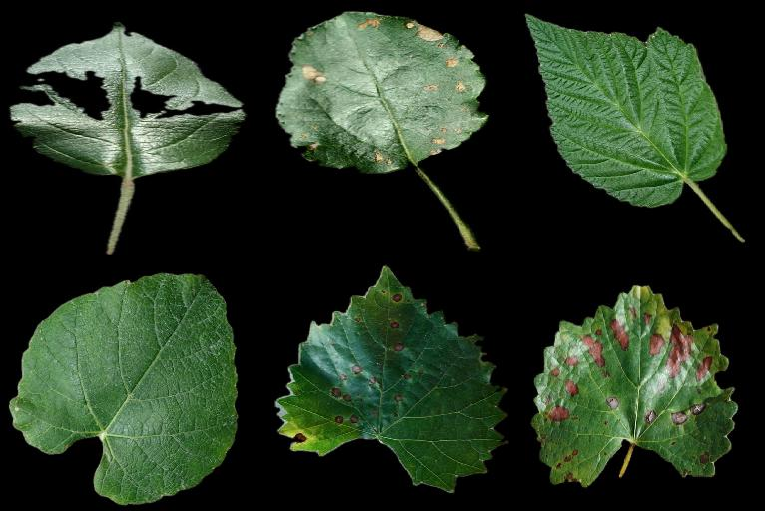
\includegraphics[width=\hsize]{figures/plant_village_subset}
	\caption{Leaf images from healthy and infected plants from the Plant Village dataset}
	\label{fig:plantvillagesubset}
\end{figure}


Firstly, the SGD algorithm is used to train a total number of $100$ epochs using the softmax regression model with mini-batch size $B=50$. Figure \ref{fig:sgd_cpu_gpu} shows the log-loss function for both, the GPU and CPU implementations. Furthermore, the model accuracy is evaluated using the final model parameters and the results can be seen in Figures \ref{fig:sgd_gpu_performance} and \ref{fig:sgd_cpu_performance}.   

\begin{figure}
	\centering
	\begin{subfigure}[b]{.5\textwidth}
		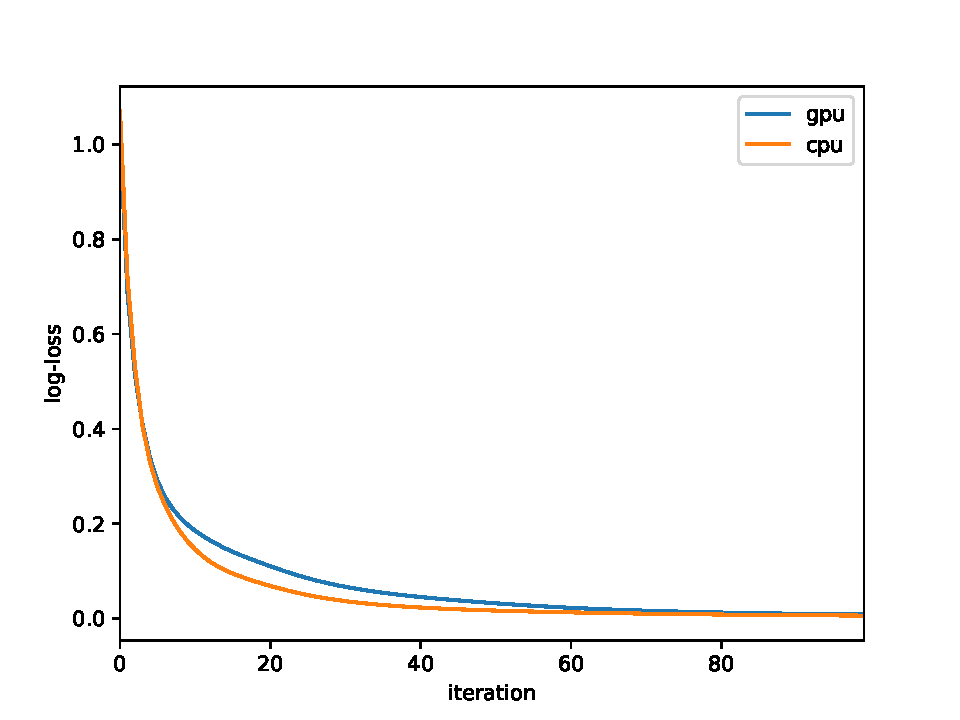
\includegraphics[width=\textwidth,height=6cm]{results/sgd_losloss}
		\caption{SGD log-loss.}
		\label{fig:sgd_cpu_gpu}
	\end{subfigure}
	~ %add desired spacing between images, e. g. ~, \quad, \qquad, \hfill etc. 
	%(or a blank line to force the subfigure onto a new line)
	\begin{subfigure}[b]{0.5\textwidth}
		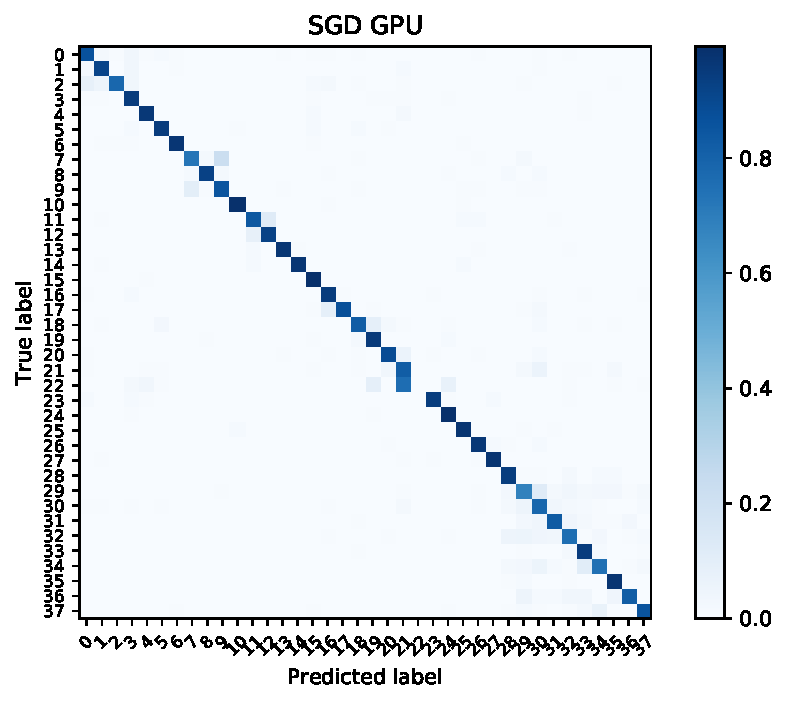
\includegraphics[width=\textwidth]{results/plants_confusion_matrix_sgd_gpu}
		\caption{SGD GPU confusion matrix.}
		\label{fig:sgd_gpu_performance}
	\end{subfigure}
	~ %add desired spacing between images, e. g. ~, \quad, \qquad, \hfill etc. 
	%(or a blank line to force the subfigure onto a new line)
	\begin{subfigure}[b]{0.5\textwidth}
		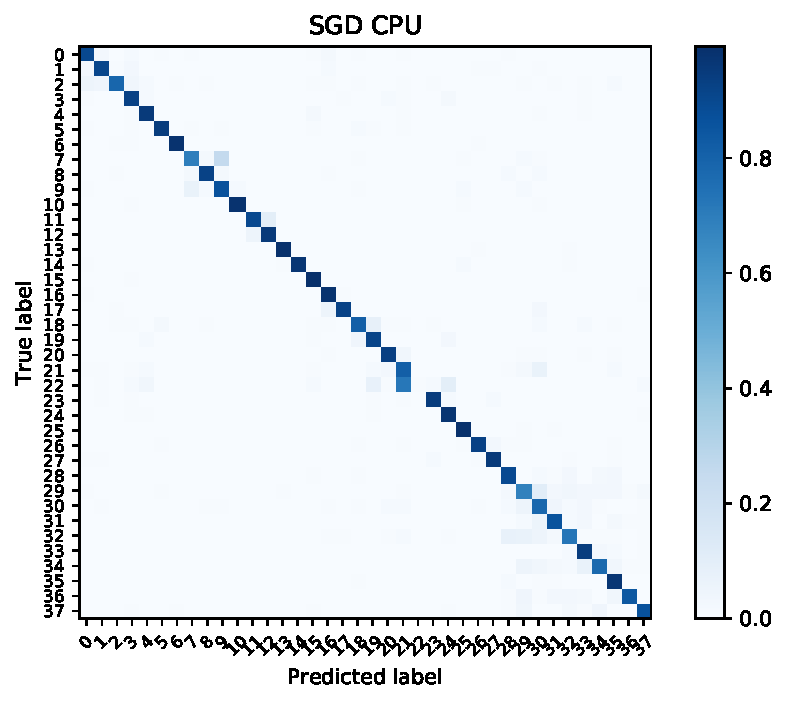
\includegraphics[width=\textwidth]{results/plants_confusion_matrix_sgd_cpu}
		\caption{SGD CPU confusion matrix.}
		\label{fig:sgd_cpu_performance}
	\end{subfigure}
	\caption{SGD performance comparison between the CPU and GPU implementations.}
\end{figure}

Secondly, GPU and multi-core CPU implementations of the SGLD algorithm are used to obtain posterior estimates of the model parameters. As opposed to SGD, most MCMC techniques such as SGLD requires a burn-in period to enter a high probability region. In this case, both implementations are tested using $10$ burn-in epochs and mini-batch size $B=50$. After that, each method runs $100$ epochs and the model parameters are kept as samples from the posterior distribution. Figure \ref{fig:sgld_cpu_gpu} shows the log-loss function for both implementations and Figures \ref{fig:sgld_gpu_performance} and \ref{fig:sgld_cpu_performance} show the achieved performance.

\begin{figure}
	\centering
	\begin{subfigure}[b]{0.5\textwidth}
		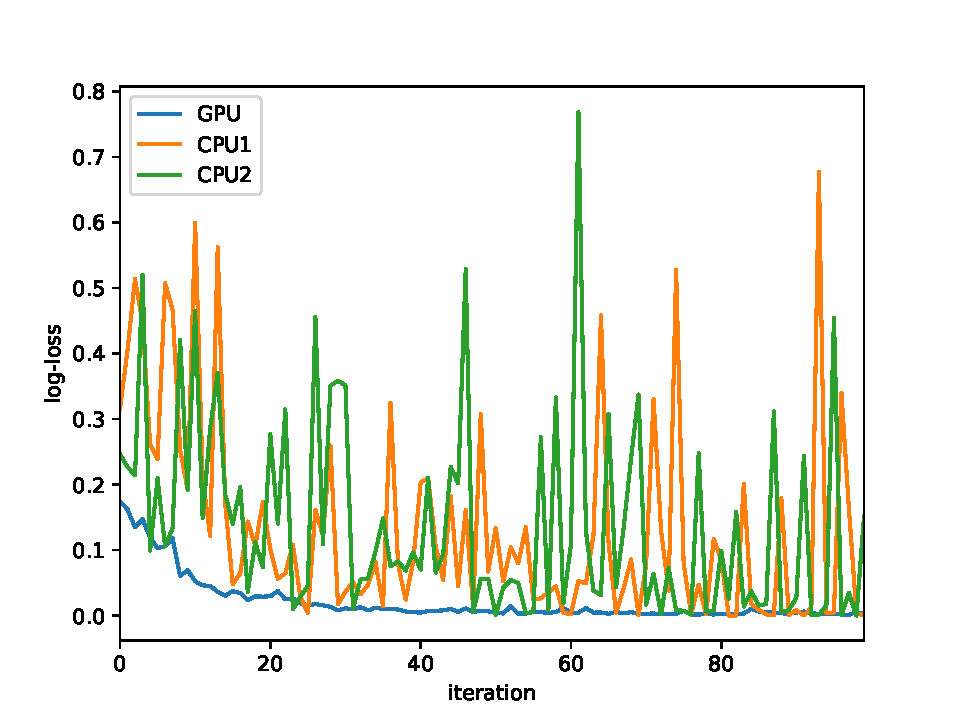
\includegraphics[width=\textwidth,height=6cm]{results/sgld_losloss}
		\caption{SGLD log-loss.}
		\label{fig:sgld_cpu_gpu}
	\end{subfigure}
	~ %add desired spacing between images, e. g. ~, \quad, \qquad, \hfill etc. 
	%(or a blank line to force the subfigure onto a new line)
	\begin{subfigure}[b]{0.5\textwidth}
		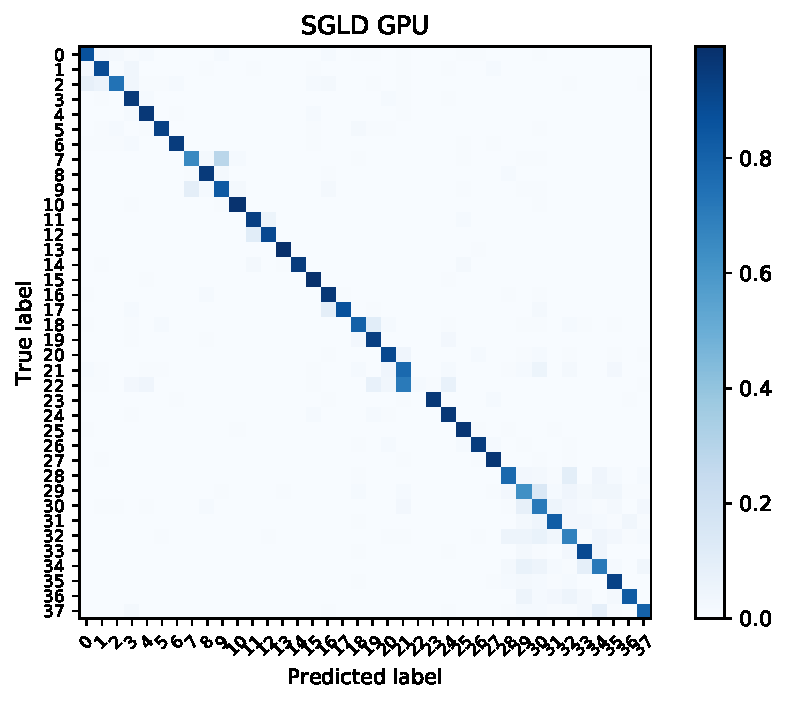
\includegraphics[width=\textwidth]{results/plants_confusion_matrix_sgld_gpu}
		\caption{SGLD GPUconfusion matrix.}
		\label{fig:sgld_gpu_performance}
	\end{subfigure}
	~ %add desired spacing between images, e. g. ~, \quad, \qquad, \hfill etc. 
	%(or a blank line to force the subfigure onto a new line)
	\begin{subfigure}[b]{0.5\textwidth}
		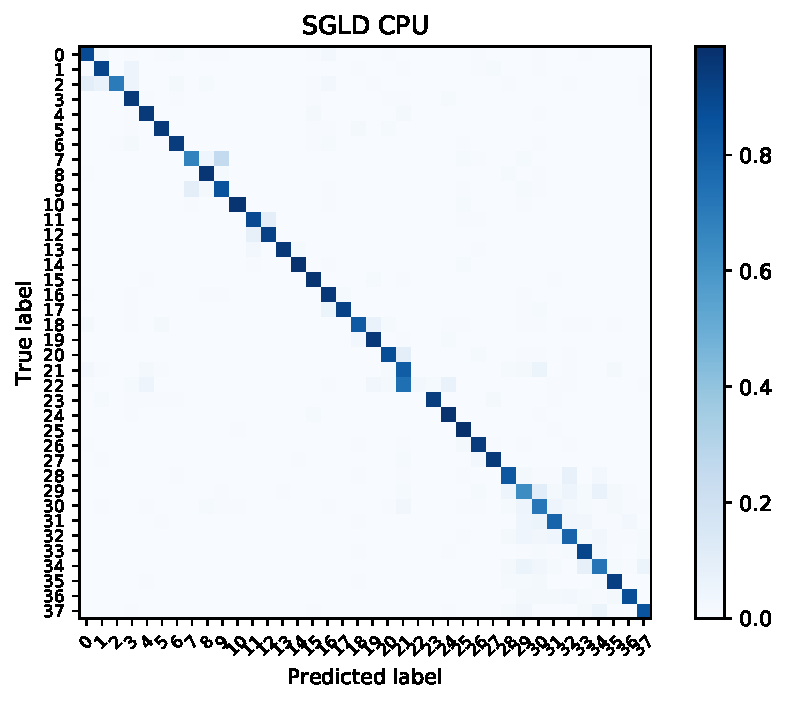
\includegraphics[width=\textwidth]{results/plants_confusion_matrix_sgld_cpu}
		\caption{SGLD CPU confusion matrix.}
		\label{fig:sgld_cpu_performance}
	\end{subfigure}
	\caption{SGLD performance comparison between the CPU and GPU implementations.}
\end{figure}

The performance of the SGLD model is evaluated using the mean of the posterior samples and the results can be seen on Table \ref{tab:performance}.


\begin{table}[h]
	\centering
	\begin{tabular}{|c|c|c|c|c|c|c|c|}
		\hline 
		& Precision & Recall & $F-1$ score & Time[s] \\ 
		\hline 
		GPU	 & $0.86$ & $0.85$ & $0.84$ & $2113.63$ \\ 
		\hline 
		CPU	 & $0.84$ & $0.83$ & $0.83$ & $16816.57$ \\ 
		\hline 
	\end{tabular}
	\caption{SGLD performance on the Plant Village test set.}
	\label{tab:performance} 
\end{table}

\clearpage
\section{Conclusions}
In this work, a novel comparison between multi-core CPU and GPU architectures for SGLD is performed. SGD is a serial algorithm that can be effectively computed using data parallel operations for large scale deep learning models. Although SGLD is an stochastic gradient MCMC method based on SGD, the algorithm can benefit from data parallel operations in a multi-core CPU architecture when the model is shallow (e.g. a single fully connected layer).  The speedups achieved with synthetic data are not compatible with other real data sets such as transfer learning data sets, which is mainly due to the size of the data batches and the model parameters. Future work will consider hybrid approaches based on multi-core CPU and multi-GPU that could also be beneficial in real life scenarios. 
\bibliographystyle{unsrt}
\bibliography{biblio}
\end{document}
